\section{Zielsetzung}
\label{sec:Zielsetzung}
In diesem Versuch sollen Gamma-Absorptionskurven von Blei und Eisen aufgenommen werden und die Absorpionskoeffizienten berechnet werden.
Außerdem soll eine Beta-Absorptionskurve von von Aluminium aufgenommen werden und daraus die Maximalenergie des Strahlers bestimmt werden.

\section{Theorie}
\label{sec:Theorie}
\subsection{Wirkungsquerschnitt und Absorptionsgesetz}
Strahlung wechselwirkt auf unterschiedliche Weise mit Materie. Wie oft eine Wechselwirkung stattfindet wird über den Wirkungsquerschnitt $\sigma$ bestimmt werden.
Hat der Absorber die Dicke $D$ und besteht aus infinitesimalen Schichten $dx$, finden nach 
\begin{align}
  dN = -N(x)n \sigma dx
\end{align}
die Reaktionen statt, wobei die Teilchenzahl um $dN$ abnimmt. $N(x)$ ist dabei die von $N_0$ abgenommene Strahlintensität.
Integriert man diese Gleichung, erhält man das Absorptionsgesetz, welches die Teilchenzahl der noch übrig gebliebenen Teilchen beschreibt
\begin{align}
  N(D) = N_0 e^{-n  \sigma D}
\end{align}
Der Exponent wird auch als Absorpionskoeffizient $\mu = n \sigma$ bezeichnet.
Für $n$ ergibt sich der Zusammenhang
\begin{align}
  n = \frac{z N_L}{V_{Mol}} = \frac{z N_L \rho}{M}
\end{align}
wobei $Z$ die Ordnungszahl, $N_L$ die Loschmidtsche Zahl, $V_{Mol}$ das Molvolumen, $M$ das Molekulargewicht und $\rho$ die Dichte ist.

\subsection{Gamma-Strahlung}
Gehen angeregte Atomkerne in einen niederenergetischen Zustand über, wird ein $\gamma -$Quant ausgesandt.
Diese Strahlung hat Wellencharakter, und für die Energie gilt dann der Zusammenhang
\begin{align}
  E = h\nu ,
\end{align}
wobei $h$ das Plancksche Wirkungsquantum ist und $\nu$ die Frequenz.
Das Linienspektrum der Gamma-Strahlung ist diskret.

Die wichtigsten Wechselwirkungen beim Durchgang durch Materie sind der Photoeffekt, der Componteffekt, und die Paarerzeugung.
Beim Photoeffekt wechselwirkt das $\gamma -$Quant mit einem Hüllenelektron, wobei es vernichtet wird. Das Elektron wird aus seiner Bindung ausgelöst.
Die Energie die es dabei erhält, ist die Energie des $\gamma -$Quants vermindert um die Bindungsenergie.
Der Photoeffekt ist bei schwere Atomen am wahrscheinlichsten, und außerdem bei den niedrigsten Quantenenergien dominierend.
Da das Elektron entfernt wird, können Elektronen aus höheren Schalen die Lücke füllen. Die Energie, die dabei frei wird, ist die Röntenstrahlung.
Beim Componteffekt wird die Strahlung an einem freien Elektron gemäß Abbildung 1 gestreuut.
\begin{figure}[H]
  \centering
  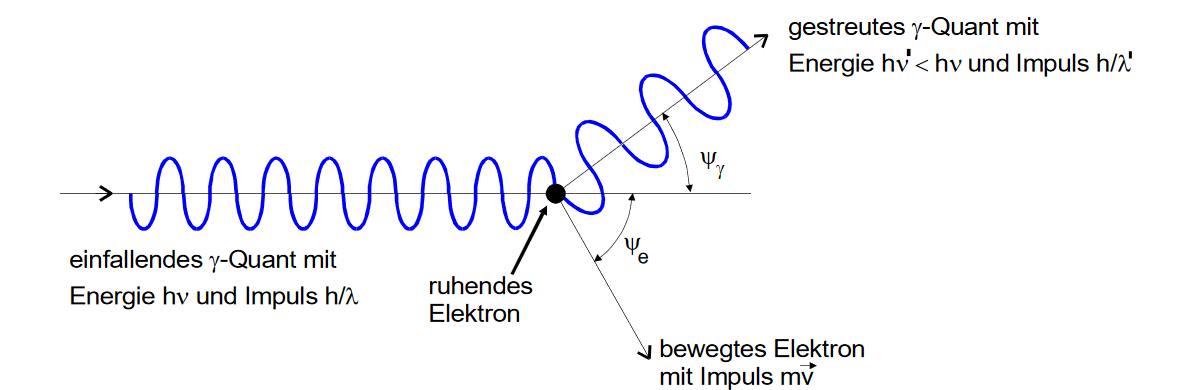
\includegraphics[width=0.8\textwidth]{compton.png}
  \caption{Darstellung der Compton-Streuung.\cite[S.5]{kent}}
  \label{fig:aufbau}
\end{figure}

\noindent Da dies eine inelastische Streuung ist, erfahren die Quanten nicht nur eine Richtungsänderung, sondern auch eine Energieänderung. 
Deshalb wird die Strahlintensität minimiert. Der Wirkungsquerschnitt für diese Streeung bestimmt sich durch
\begin{align}
  \sigma_{com} = 2 \pi r_e^2 \left(\frac{1+\epsilon}{\epsilon^2} \left[\frac{2(1+\epsilon)}{1+2\epsilon}-\frac{1}{\epsilon} ln(1+2\epsilon) \right]
                + \frac{1}{2\epsilon} ln(1+2\epsilon) - \frac{1+3\epsilon}{(1+2\epsilon)^2} \right)
\end{align}
Hierbei ist  $\epsilon = E_{\gamma}/(m_0 c^2)$, und $r_e = \frac{e_0^2}{4 \pi \epsilon_0 m_0 c^2} = 2,82 \cdot 10^{-15}$m der klassische Elektronenradius, mit $e_0$ die Elementarladung und $\epsilon_0$ die Influenzkonstante.
Der Absorpionskoeffizient wird definiert durch
\begin{align}
  \mu_{com} =\frac{z N_A \rho}{M} \sigma_{com}.
\end{align}
Dieser Effekt tritt bei mittleren Energien,also ab 200 $\si{\keV}$ auf.
Ist die Energie der Gammastrahlung größer als die doppelte Ruhemasse eines Elektrons, tritt die Paarerzeugung ein.
Hierbei wird das Quant vernichtet und dabei entsteht ein Elektron und ein Positron.
Diese Wechselwirkung tritt ab einer Energie von 1 $\si{\MeV}$ auf.
Ein Kurvenverlauf für die Energieabhängigkeit der Absorptionskoeffizienten ist in Abbildung 2 zu sehen.
\begin{figure}[H]
  \centering
  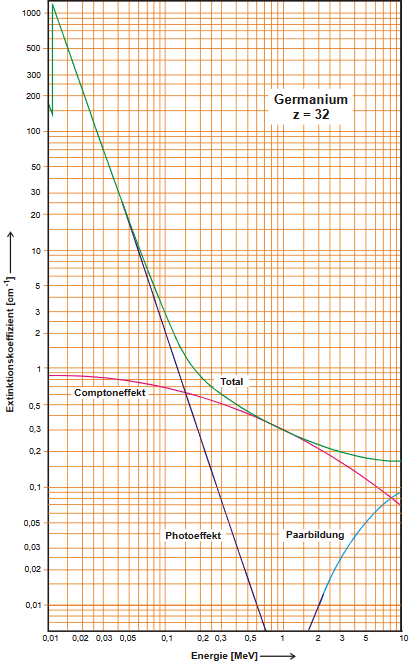
\includegraphics[width=0.8\textwidth]{kurve.png}
  \caption{Kurvenverläuge für die Energieabhängigkeit der Absorpionskoeffizienten für die 3 Wechselwirkungen und der Totaleffekt.\cite[S.7]{kent}}
  \label{fig:aufbau}
\end{figure}

\subsection{Beta-Strahlung}
Beta-Strahlung entsteht wenn ein Atomkern zerfällt. Beim $\beta^{-}$-Zerfall entsteht ein Proton, ein Elektron und ein Antineutrino, nachdem ein Neutron zerfällt.
Beim $\beta^{+}$-Zerfall zerfällt ein Proton in ein Neutron, ein Positron und ein Neutrino. 
Hier ist das Energiespektrum kontinuierlich.
Es gibt drei Wechselwirkungsprozesse mit Materie.
Die Elastische Streuung am Atomkern ist im Grunde die Rutherford-Streuung. Im Coulomb-feld der Kerne werden die $\beta-$Teilchen abgelenkt, wobei die Strahlintensität abfällt.

\noindent Bei der inelastischen Streuung am Atomkern erfahren die Teilchen eine Beschleunigung. Dabei wird Energie abgegeben, welche die Teilchen abbremst; sie wird somit auch als Bremsstrahlung bezeichnet.

\noindent Die inelastische Streuung an den Elektronen der Materie führt zu Ionisation und Anregung der Absorberatome. Es können viele solcher Prozesse hintereinander ausgeführt werden, da nur wenig Energie verbraucht wird. 

\noindent Eine Absorptionskurve für die $\beta-$Strahlung ist in Abbildung 3 gegeben. 
Hier ist der Logarithmus der Strahlintensität gegen die Massenbelegung 
\begin{align}
R = \rho D
\end{align} aufgetragen. Aus der Kurve kann die maximale Reichweite $R_{max}$ bestimmt werden.
Daraus kann wiederum die maximale Energie über die Beziehung
\begin{align}
  E_{max} = 1,92 \sqrt{R_{max}^2 + 0,22 R_{max}}
\end{align}
berechnet werden.
\begin{figure}[H]
  \centering
  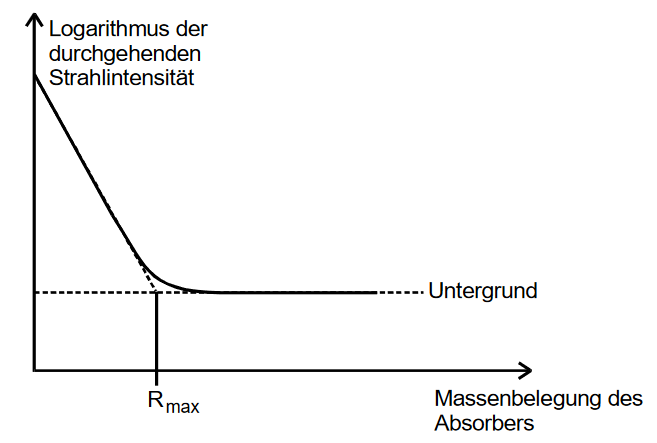
\includegraphics[width=0.8\textwidth]{beta.png}
  \caption{Absorptionskurve für die Beta-Strahlung.\cite[S.12]{kent}}
  \label{fig:aufbau}
\end{figure}
